% ============================================================
% IE UNIVERSITY - BACHELOR IN APPLIED MATHEMATICS
% Machine Learning group project: final report (official BAM template)
% Compile with PDFLaTeX. Figures in ./figures and ./eda.
% ============================================================
\documentclass[clean,twocolumn]{bam-project}

\BAMtitle{Learning Where: Country Classification from Crowd-Sourced Street-Level Imagery}
\BAMshorttitle{Street-Level Country Classification}
\BAMcourse{Machine Learning -- Group Project}
\BAMteam{Kwanhyung Kim\\[0.2em]Guillermo Gonzalez}
\BAMinstructors{Nacho Molina Clemente}
\BAMsubmissiondate{\today}

\graphicspath{{figures/}{eda/}}
\captionsetup{font=small,labelfont=bf,labelsep=period,skip=4pt}
\newcommand{\tsh}{test\textsubscript{shared}}
\newcommand{\vsh}{val\textsubscript{shared}}
\newcommand{\pp}{\,pp}
\newcommand{\pending}[1]{\textcolor{red}{[#1]}}

\begin{document}

\makebamtitle

\begin{BAMabstract}
We ask to what extent a convolutional neural network (CNN) trained on crowd-sourced street-level
imagery learns country cues that transfer to photographers it has never seen. On 32 countries of
OpenStreetView-5M (OSV-5M) we assign \emph{contributors}, not images, to training, validation and test,
and add a second test set of new trips by training contributors; the difference between the two, the
contributor gap $\Delta$, measures how much accuracy depends on having seen the photographer. A
colour/HOG nearest-neighbour baseline reaches 5.6\% balanced accuracy (chance 3.1\%), a linear probe on
frozen ImageNet features 13.5\%, a partially fine-tuned ResNet-18 30.7\% and an end-to-end fine-tuned ResNet-18 31.9\% on unseen contributors. Frozen
features show no gap; fitting the network to the training contributors creates one ($+7.4$\pp), it
grows with more images of the same contributors and with a contributor's number of training images, and
retrieval of the same photographer explains most of it. Hiding the bottom 20\% of the frame (bonnet,
dashboard) at test time removes 4.3\pp\ of the gap, and training with fingerprint removal changes the gap by $-$2.1\pp\ [$-$3.3, $-$0.9] (to $+$3.1\pp) at a cost of 3.6\pp\ [2.8, 4.5] on unseen contributors. The network learns countries, but part of its accuracy on familiar
photographers is the camera.
\end{BAMabstract}

\section{Introduction}
\subsection{Research Question}
To what extent can a convolutional neural network (CNN) trained end-to-end on crowd-sourced
street-level imagery (OpenStreetView-5M) learn country-discriminative visual features that generalise
beyond the contributors seen during training?

\subsection{Motivation}
GeoGuessr is an online geography game that drops players into a random street-view location and
challenges them to guess where it is (\emph{GeoGuessr}). As travel enthusiasts who grew up as
third-culture individuals, we have always been intrigued by different countries, and became interested in
how neural networks can identify trends in dash-camera images from across the world. Crowd-sourced data
raise a question that benchmark accuracy hides: \emph{whose} images does a model recognise? Photos by
one contributor share the bonnet, windscreen reflections and colour profile of one camera (Luk\'a\v{s}
et al.), so a model can score well by recognising photographers rather than countries, a known form of
shortcut learning (Geirhos et al.; Torralba and Efros; Zech et al.).

\subsection{Related Work}
Image geolocation has moved from retrieval to classification and then to large pretrained models.
IM2GPS matched photos to their nearest geotagged neighbours using hand-crafted features (Hays and
Efros), PlaNet classified photos into geographic cells with a CNN (Weyand et al.), and GeoCLIP
(Vivanco Cepeda et al.) and PIGEON build on large-scale image--text pretraining; PIGEON reaches about
92\% country accuracy on Street View and beats top GeoGuessr players (Haas et al.). On OSV-5M, the
authors' best model, a fine-tuned ViT-L/14, reaches 68.0\% country accuracy against 48.9\% for humans
(Astruc et al.). These benchmarks separate training and test images by location and by sequence but
not by photographer, and the OSV-5M authors note that the same vehicle can appear in both sets. Our
goal differs: rather than maximising accuracy, we measure how much of it survives for contributors a
model has never seen, with a small model trained on our own hardware.

\section{Data}
\subsection{Dataset}
We use OpenStreetView-5M, a crowd-sourced Mapillary collection of 4.89M training and 210k test images
from 225 countries (CC BY-SA 4.0) (Astruc et al.). Each image comes with GPS coordinates, country,
capture time, sequence (trip) and contributor IDs. Nearly all images are forward-facing road views, and
the contributor IDs make a contributor-disjoint split possible.

\subsection{Exploratory Data Analysis}
The training set is imbalanced at two levels. By country, the United States accounts for 24.9\% of
images and the ten largest countries for 58.3\%. By contributor, the median contributor supplied 8
images, while the top 100 of 20{,}394 supplied 45.7\%. The effective number of contributors,
$N_{\text{eff}}=1/\sum_i p_i^2$ with $p_i$ contributor $i$'s share of a country's images, is only 14 for the
United States despite 2{,}500 contributors and 1.1 for Pakistan, where one contributor took 95\% of the
images (Figure~\ref{fig:eda}). 98.2\% of the official test images come from contributors who also appear
in training, so we use only the official training split and build our own contributor-disjoint
evaluation. Figure~\ref{fig:samephot} shows why this matters: four trips by the same photographer share
the camera's colour, field of view and bonnet, even on different roads. The EDA and the pilot study in Section~\ref{sec:pilot} were run with the code in
\url{https://github.com/LaGuadana/geo_cnn}.

\begin{figure*}[!t]
\centering
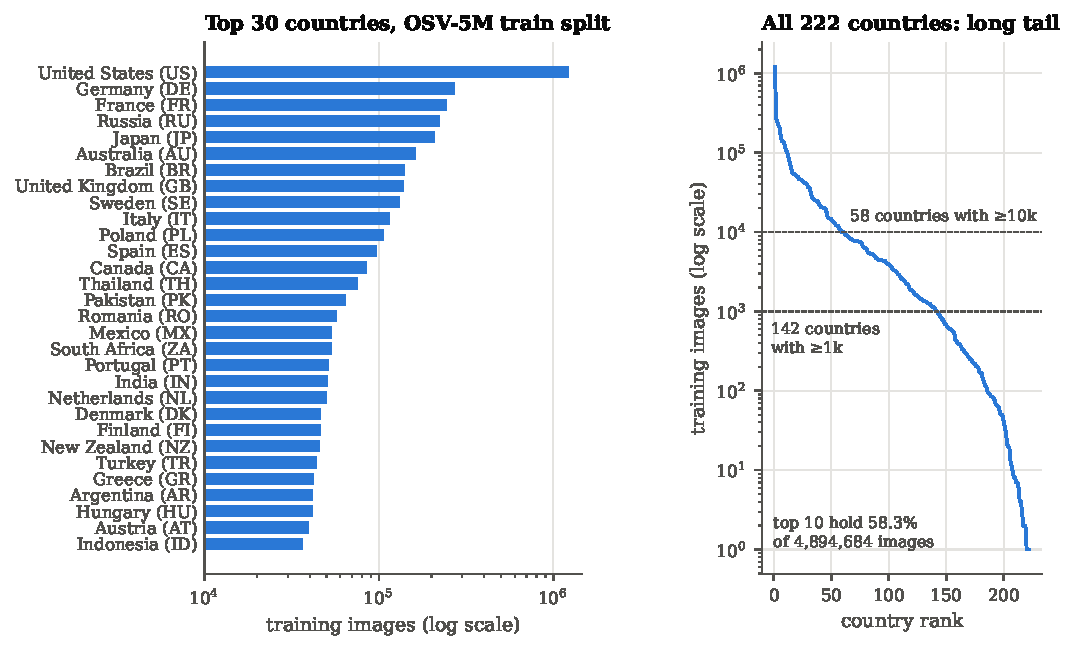
\includegraphics[width=0.62\textwidth]{fig_a_country_counts}\\[4pt]
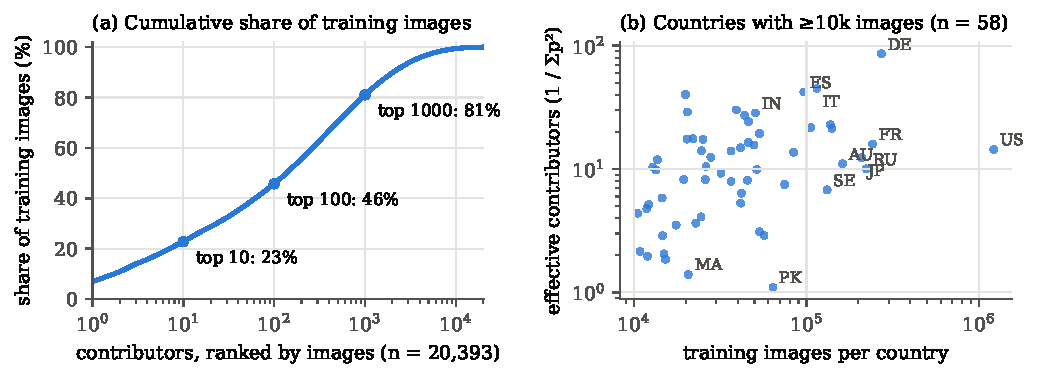
\includegraphics[width=0.9\textwidth]{fig_g_contributors}
\caption{Imbalance in the OSV-5M training split. Top: images per country for the 30 largest countries
(left) and for all 222 countries by rank (right); the ten largest hold 58.3\% of the 4.89M images.
Bottom: (a) cumulative share of training images by contributor rank, where the top 100 contributors
supply 46\%; (b) effective number of contributors, $1/\sum_i p_i^2$, against training images for the
58 countries with at least 10{,}000 images.}
\label{fig:eda}
\end{figure*}

\begin{figure*}[!t]
\centering
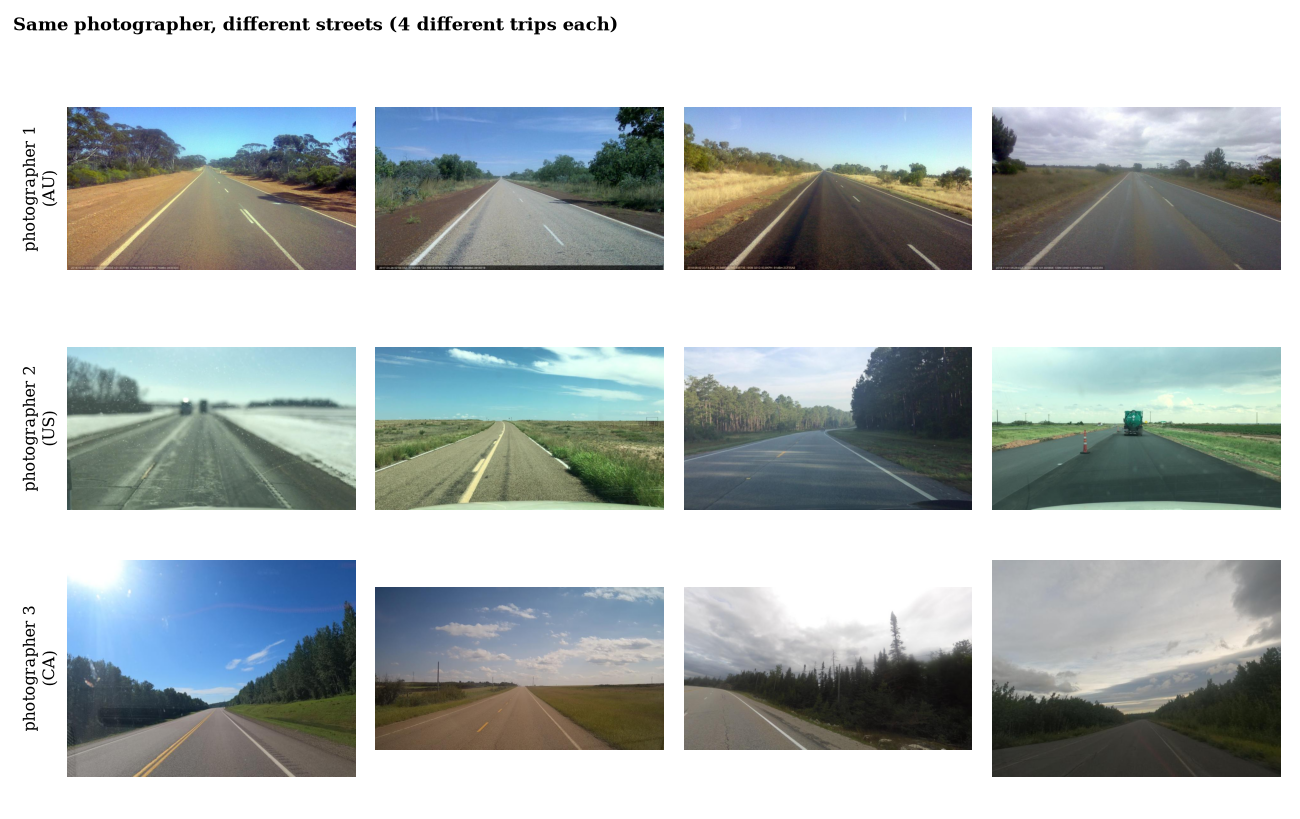
\includegraphics[width=0.78\textwidth]{fig_f_same_photographer}
\caption{Same photographer, different streets: four trips each by three OSV-5M contributors (Australia,
United States, Canada). Photos: OSV-5M / Mapillary contributors, CC BY-SA 4.0.}
\label{fig:samephot}
\end{figure*}


\subsection{Subset, Splits and Preprocessing}
We keep the 32 countries with at least 200 contributors. Contributors are assigned 70/10/20 to
training, validation and test, stratified by each contributor's main country. Inside the training
contributors, whole groups of images linked by the same sequence or the same contributor-specific
$0.1^\circ$ cell ($\approx$11\,km) are held out as \vsh\ and \tsh: new trips and places by photographers the
model has seen. Per split and country, a fixed budget is filled by water-filling: every contributor
gets at most $c$ images, $c$ as large as the budget allows, taken round-robin over its trips
(Table~\ref{tab:data}). The selection script checks that no contributor is shared between training,
validation and test and that no sequence is shared between training and any evaluation split. Images
are centre-cropped to 4:3, since the aspect ratio (4:3 or 16:9) is itself a camera property, and stored
at $128\times170$ pixels. Single images are fetched from the remote archives by HTTP range requests, so
the 139{,}696-image subset takes 1.0\,GB instead of about 245\,GB of archives.

\begin{table*}[!t]
\centering\small
\caption{The 32-country subset. test and \tsh\ differ only in whether the photographer is in the training set.}
\label{tab:data}
\setlength{\tabcolsep}{3.5pt}\footnotesize
\begin{tabular}{@{}lrrrl@{}}
\toprule
split & images & contributors & per country & role \\
\midrule
train & 101{,}578 & 11{,}132 & 3{,}200 (ET 2{,}649, MY 2{,}929) & training \\
val & 6{,}400 & 1{,}521 & 200 & model selection, unseen contributors \\
test & 12{,}800 & 3{,}043 & 400 & \textbf{unseen contributors} \\
\vsh & 6{,}359 & 2{,}089 & $\le$200 & new trips of training contributors \\
\tsh & 12{,}559 & 3{,}037 & $\le$400 & \textbf{seen contributors, new trips} \\
extra chunks 1--3 & $+$261{,}572 & & uneven (US 60{,}637; ET, MY 0) & more data, $\le$100 per contributor \\
\bottomrule
\end{tabular}
\end{table*}

\section{Methodology}
\subsection{Evaluation}
Balanced accuracy (BA), the mean per-class recall (chance 3.1\%), equals top-1 accuracy on the balanced
test set. Accuracy on test answers the research question; the contributor gap
$\Delta=\mathrm{BA}(\text{\tsh})-\mathrm{BA}(\text{test})$ measures how much accuracy depends on having
seen the photographer. All 95\% confidence intervals (CIs) come from a bootstrap that resamples
contributors rather than images, because one photographer's photos are correlated (Field and Welsh);
differences between models use paired draws on the same images.

\subsection{Models}
All CNNs are ResNet-18 (He et al.): a $7\times7$ stem and four stages of residual blocks ending in a
512-dimensional feature (a $4\times6$ map average-pooled at our input size), dropout 0.2 and a 32-way
output layer (11.2M parameters). Images are never flipped, because mirroring swaps the driving side.
\begin{enumerate}[label=(\arabic*),leftmargin=*]
\item \emph{Classical baseline} (Hays and Efros): HSV colour histogram and HOG features (Dalal and
Triggs), 2{,}268 dimensions, reduced by PCA to 256 and classified by distance-weighted 15-nearest
neighbours (cosine), on 9{,}600 training images.
\item \emph{Linear probe}: $L_2$-regularised softmax regression on frozen ImageNet features (Deng et
al.) of the same 9{,}600 images.
\item \emph{Partial fine-tune}: from the probe, the last two stages and the output layer are trained on
the 101{,}578 training images on a laptop CPU (stem and stages 1--2 frozen).
\item \emph{More data}: model (3) continues on three further chunks of about 87k images each (363k
distinct images in total). The final chunk is our released checkpoint.
\item \emph{End-to-end fine-tune}: all layers of the ImageNet ResNet-18 trained on the 101{,}578
training images on a laptop GPU, \emph{once with and once without fingerprint removal}, otherwise
identical (same seed, data order and schedule).
\item \emph{$k$-NN on learned features} of (2) and (4): shows whether predictions rely on finding
photos by the same photographer.
\end{enumerate}

\subsection{Removing the Camera Fingerprint}
The proposal planned to mask pixels that stay constant across a contributor's photos, but no pixel had
an across-photo standard deviation below 15 for any of the 60 largest contributors: bonnets reflect the
sky, contributors change cars and mounts, and the most stable regions were road, snow and sky, which are
country cues. Fingerprint removal therefore blanks the bottom 20\% of every image to the ImageNet mean
colour (blanking rather than cropping keeps the geometry fixed) and, during training, re-encodes images
as JPEG at quality 30--95 and jitters white balance ($\pm15\%$), brightness, contrast and saturation
($\pm25\%$), but not hue, since road-marking colour is a country cue. We also apply the blanking to
trained standard models \emph{at test time only}, which needs no retraining.

\subsection{Training Configuration}
\begin{table*}[!t]
\centering\small
\caption{Training configuration. val is the contributor-disjoint validation set.}
\label{tab:config}
\begin{tabularx}{\textwidth}{@{}l>{\raggedright}X>{\raggedright}X>{\raggedright}X>{\raggedright\arraybackslash}X@{}}
\toprule
 & (1) Classical / (2) Probe & (3) Partial fine-tune & (4) More data & (5) End-to-end \\
\midrule
Trained layers & -- / output layer & stages 3--4 + output & same as (3) & all \\
Training images & 9{,}600 & 101{,}578 & +87k per chunk (363k) & 101{,}578 \\
Optimiser & -- / L-BFGS & SGD, Nesterov 0.9, batch 64 & same & SGD, Nesterov 0.9, batch 256 \\
Learning rate & -- & 0.02 per 256, warm-up, cosine & 0.01 (chunk 1), 0.004 & 0.01 per 256, 1 epoch warm-up, cosine \\
Regularisation & -- / $L_2$ penalty & weight decay $10^{-4}$, dropout 0.2, label smoothing 0.1, random crops, no flips & same + class weights & same as (3) \\
Length & -- & 24 epochs of 20{,}480 & one pass per chunk & 6 epochs \\
Tuned on val & $k$, distance / $L_2\in[10^{-4},10^{-2}]$ & best epoch & best epoch & best epoch \\
Hardware, time & CPU, $\approx$7 min & 4-core CPU, 7.7\,h & CPU, $\approx$1.8\,h per chunk & Apple M5 GPU, bf16, $\approx$13--20 min per epoch \\
\bottomrule
\end{tabularx}
\end{table*}

For the probe, raising the $L_2$ penalty from $10^{-4}$ to $10^{-2}$ lowers training accuracy from 48.7\%
to 34.3\% but raises validation accuracy from 12.8\% to 16.7\%, a clear bias--variance trade-off; the
optimum lies at the edge of the grid, so the probe slightly underestimates frozen features. For the
end-to-end runs, the training script's default (0.02 per 256 with a ten-times larger rate for the output
layer) collapsed to chance accuracy in a trial and was replaced by 0.01 for all layers. The runs were
planned for 8 epochs; after 4 epochs, memory pressure from running both at once on a 16\,GB laptop made
us finish them one after the other with the cosine schedule shortened to 6 epochs, identically for both.

\section{Results}
\subsection{Pilot Study}\label{sec:pilot}
Before building the 32-country subset, we balanced the ten most frequent countries of one OSV-5M shard to
162 images each and compared contributors shared or disjoint between training and test
(Table~\ref{tab:pilot}). Both models lose close to half their accuracy once contributors are disjoint;
recall for Australia, where most images come from one contributor, drops from 81\% to 19\%. This made a
contributor-disjoint protocol the basis of our comparison.

\begin{table}[!t]
\centering\small
\caption{Pilot study: top-1 accuracy on ten balanced countries from one OSV-5M shard (chance 10\%; about $\pm5$ percentage points).}
\label{tab:pilot}
\resizebox{\columnwidth}{!}{%
\begin{tabular}{@{}lcc@{}}
\toprule
Model & Contributors shared & Contributors disjoint \\
\midrule
Majority class & 9.9\% & 10.0\% \\
HSV histograms + logistic regression & 37.3\% & 19.3\% \\
Frozen ResNet-18 + logistic regression & 48.1\% & 28.1\% \\
\bottomrule
\end{tabular}}
\end{table}

\subsection{Model Comparison}
\begin{table*}[!t]
\centering\small
\caption{Balanced accuracy (\%) on unseen (test) and seen (\tsh) contributors with 95\%
contributor-bootstrap CIs, the gap $\Delta$, top-3 accuracy on test and the median distance (km) from
misclassified test images to the predicted country. The 15-NN rows report top-1 accuracy.}
\label{tab:main}
\setlength{\tabcolsep}{4pt}
\begin{tabular}{@{}llllrr@{}}
\toprule
Model & test & \tsh & $\Delta$ (pp) & top-3 & km \\
\midrule
(1) Classical & 5.6 [5.1, 6.2] & 6.5 & $+$0.9 [0.0, 1.7] & -- & 6{,}252 \\
(2) Linear probe & 13.5 [12.8, 14.3] & 13.7 & $+$0.2 [$-$1.1, 1.4] & 29.4 & 5{,}543 \\
(3) Partial fine-tune & 28.7 [27.5, 29.8] & 34.5 & $+$5.8 [4.1, 7.5] & 51.1 & 2{,}439 \\
(4) + chunk 1 & 29.8 [28.6, 31.0] & 36.8 & $+$7.0 [5.2, 8.8] & 51.7 & 2{,}679 \\
\phantom{(4)} + chunk 2 & 30.1 [28.9, 31.3] & 37.7 & $+$7.6 [5.8, 9.4] & 51.7 & 2{,}852 \\
\phantom{(4)} + chunk 3 & 30.7 [29.4, 31.9] & 38.0 & $+$7.4 [5.6, 9.2] & 52.4 & 2{,}865 \\
\phantom{(4)} + chunk 3, bottom blanked at test & 20.9 [20.0, 21.8] & 23.9 & $+$3.0 [1.6, 4.5] & 40.0 & \\
\midrule
(5) End-to-end, standard & 31.9 [30.6, 33.1] & 37.0 & $+$5.2 [3.4, 6.9] & 54.2 & 2{,}457 \\
\phantom{(5)} standard, bottom blanked at test & 22.6 [21.7, 23.5] & 25.3 & $+$2.7 [1.3, 4.2] & 42.7 &  \\
(5) End-to-end, fingerprint removal & 28.2 [27.1, 29.3] & 31.3 & $+$3.1 [1.3, 4.8] & 50.3 & 2{,}743 \\
\midrule
(6) 15-NN on (2) & 9.7 & 11.5 & $+$1.8 & & \\
(6) 15-NN on (4) & 25.3 & 32.8 & $+$7.5 & & \\
\bottomrule
\end{tabular}
\end{table*}

Table~\ref{tab:main} and Figure~\ref{fig:scaling}a summarise the comparison. The classical baseline
reaches 5.6\% BA, less than twice chance, with errors a median 6{,}252\,km from the predicted country.
Frozen ImageNet features more than double this (13.5\%), and fine-tuning the upper network doubles it
again (28.7\%): the median error distance falls from 5{,}543 to 2{,}439\,km and top-3 accuracy rises
from 29.4\% to 51.1\%. The 15-NN classifier on the same features shows the same jump (9.7\% to 25.3\%):
fine-tuning reorganises the feature space so that images of one country lie close together.
Training all layers end to end on the same 101{,}578 images reaches 31.9\% on unseen contributors, $+$1.2\pp\ [0.4, 1.9] against the final partially fine-tuned model that saw 3.6 times more images, with a gap of $+$5.2\pp\ [3.4, 6.9] against $+$7.4\pp\ (paired change $-$2.2\pp\ [$-$3.3, $-$1.1]).

The contributor gap behaves differently. It is within 1\pp\ of zero for the classical baseline and the
probe, $+5.8$\pp\ after fine-tuning and $+7.4$\pp\ after the extra data. Tripling the distinct training
images adds 2.0\pp\ [1.4, 2.5] on unseen contributors but 3.5\pp\ on seen ones, so $\Delta$ grows by a
paired 1.6\pp\ [0.6, 2.5]: the extra images are mostly new trips of contributors already in training, so
the models overfit to photographers rather than to individual images.

\begin{figure*}[!t]
\centering
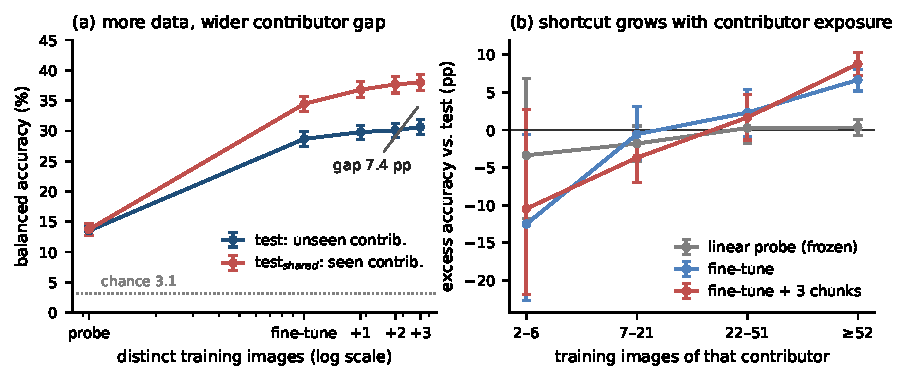
\includegraphics[width=0.95\textwidth]{scaling_decomposition}
\caption{(a) Accuracy on seen contributors (\tsh) grows faster with more training images than accuracy
on unseen ones (test). (b) Excess accuracy on new trips of seen contributors, grouped by how many of
their images were in training, with 95\% CIs. The probe stays flat, while the fine-tuned models gain up
to 8.8\pp\ for the most-seen contributors.}
\label{fig:scaling}
\end{figure*}

\subsection{Which Countries Are Hard?}
Figure~\ref{fig:countries}a breaks accuracy down by country. For the end-to-end model, recall on unseen
contributors ranges from 9.5\% for France to 63.3\% for Ethiopia, followed by India (58.0\%), Taiwan
(54.5\%) and Japan (54.3\%); the hardest countries are France, Czechia (13.3\%), Poland (14.0\%) and Portugal
(18.0\%), and the eleven hardest are all European. The ranking is stable across models: the final partially
fine-tuned model also goes from France (8\%) to Ethiopia (69\%). Easy countries are those without a
look-alike in the class set. Ethiopia is the only African country, and its 400 test images come from 38
photographers, none dominant (largest share 4\%), so its recall is not a memorised camera; its precision
(67\%) matches its recall, so it is not a default guess either. Hard countries are surrounded by similar
ones: Austria is predicted as Switzerland for 80 of its 400 images (and Switzerland as Austria for 53),
Canada as the United States for 73, and Belgium, Germany and Denmark as the Netherlands for 38 to 57
each. We infer that at $128\times170$ pixels the network relies mostly on coarse scene properties
(vegetation, terrain, building density, road layout) that are shared within a region, and much less on
fine cues that separate neighbours, such as the text and colour of signs, licence plates or bollards,
which are only a few pixels large at this resolution.

End-to-end training does not raise all countries equally. Against the final partially fine-tuned model it
gains most in Sweden ($+11.5$\pp), the United States ($+9.5$), Germany ($+9.2$) and Brazil ($+6.5$), and loses
most in Russia ($-6.8$), Taiwan ($-6.0$), Ethiopia ($-5.3$) and the Netherlands ($-5.0$). The countries that gain
are those with the most extra images in the data chunks, which inverse-frequency class weights had
down-weighted, and Ethiopia, which loses, had been up-weighted about twelve-fold and replayed at every
stage. Part of the per-country profile of the earlier model therefore reflects its training objective, not
only what the images show.

\subsection{What the Errors Look Like}
Errors carry geographic structure that grows with how much of the network is trained
(Table~\ref{tab:errors}). If a wrong answer were a random other country, 40 to 43\% of errors would stay in
the true country's world region (Europe, the Americas, Asia, Oceania, Africa). The classical baseline is
close to that (44\%), frozen features slightly above (48\%), and the fine-tuned networks well above (59 to
62\%). Driving side is the clearest learned cue: of the 2{,}800 test images from the seven left-hand-traffic
countries (Australia, India, Indonesia, Japan, Malaysia, Thailand, United Kingdom), the classical baseline
assigns 32\% to a left-hand-traffic country, frozen features 43\%, and every fine-tuned model 68 to 70\%,
against 22\% for a uniform guess. This is why we never flip images: a mirrored training image would teach
the opposite side. Most confusions are within one driving side and one region (India and Indonesia,
Malaysia and Indonesia, Japan and Taiwan), and the median error lands 2{,}457\,km from the predicted
country for the end-to-end model, against 2{,}865\,km for the final partially fine-tuned model and
5{,}543\,km for frozen features.

\begin{table*}[!t]
\centering\small
\caption{Structure of the errors on test (unseen contributors). ``Same region'': share of misclassified
images whose predicted country lies in the same world region as the true one; chance assumes a uniform
wrong answer. ``Left $\to$ left'': share of images from left-hand-traffic countries assigned to a
left-hand-traffic country (uniform guess 22\%).}
\label{tab:errors}
\begin{tabular}{@{}lrrrr@{}}
\toprule
Model & error rate & same region (chance) & left $\to$ left & median error (km) \\
\midrule
(1) Classical & 94.4\% & 44.4\% (39.7\%) & 32.4\% & 6{,}252 \\
(2) Linear probe & 86.5\% & 47.8\% (41.0\%) & 43.3\% & 5{,}543 \\
(4) Partial fine-tune + 3 chunks & 69.3\% & 59.1\% (42.8\%) & 68.4\% & 2{,}865 \\
(5) End-to-end, standard & 68.1\% & 62.1\% (42.6\%) & 70.3\% & 2{,}457 \\
(5) End-to-end, fingerprint removal & 71.8\% & 59.1\% (42.5\%) & 69.6\% & 2{,}743 \\
\bottomrule
\end{tabular}
\end{table*}

\begin{figure*}[!t]
\centering
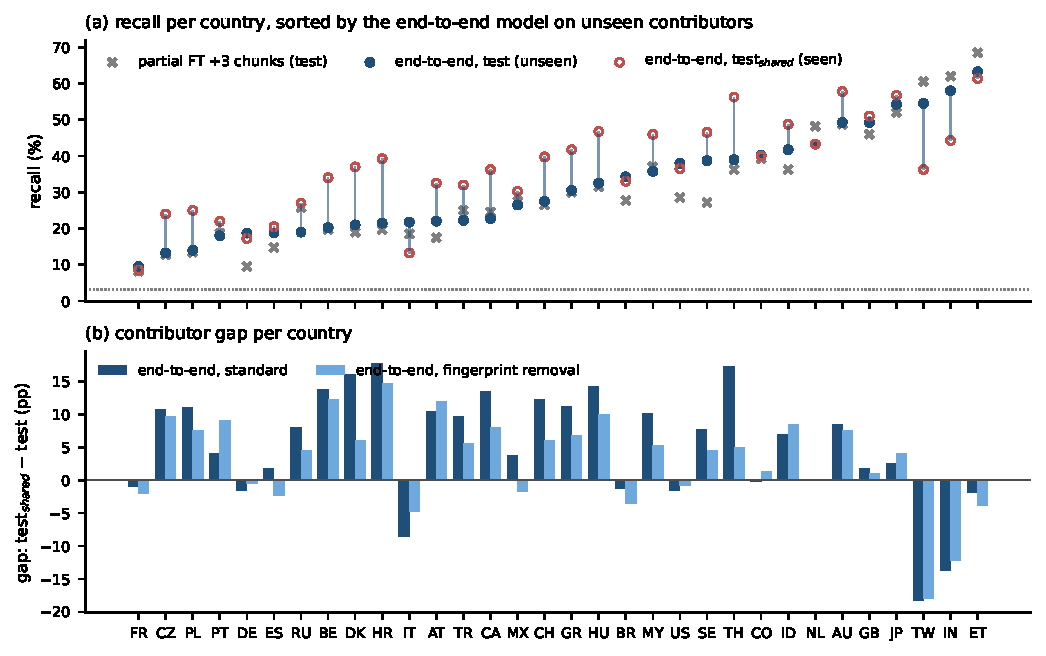
\includegraphics[width=\textwidth]{fig_countries}
\caption{(a) Recall per country (ISO codes), sorted by the end-to-end model's recall on unseen
contributors (filled); lines connect it with recall on seen contributors (open); crosses show the final
partially fine-tuned model. (b) Per-country contributor gap of the end-to-end model without and with
fingerprint removal. With 400 test images per country (272--400 in \tsh), each value carries roughly
$\pm4$--5\pp\ of sampling uncertainty.}
\label{fig:countries}
\end{figure*}

\section{Where the Contributor Gap Comes From}
\paragraph{Exposure.} If seen contributors simply photographed easier places, accuracy on their new trips
would not depend on how many of their images were in training. We group \tsh\ contributors by their
number of training images and compute the excess accuracy
\begin{equation}
E_B=\frac{1}{|B|}\sum_{i\in B}\big(\mathbf{1}[\hat y_i=y_i]-a_{c(i)}\big),
\end{equation}
where $a_c$ is the model's accuracy on country $c$ in test, so that each image is compared with its own
country's level for unseen photographers. For the probe, $E_B$ stays flat ($+0.3$\pp\ [$-0.7$, 1.4] at 52 or
more images); for the final partially fine-tuned model it rises to $+8.8$\pp\ [7.3, 10.3] for contributors
with 52 or more training images (84\% of \tsh; Figure~\ref{fig:scaling}b). The end-to-end models were
trained on the 101{,}578 manifest images only, where a seen contributor has between 2 and 556 images
(median 12), so we bin them on those counts (Figure~\ref{fig:exposure}). The standard end-to-end model shows
the same dose--response: $-3.7$\pp\ [$-6.2$, $-1.2$] for contributors with 2--5 training images, $+0.5$ and
$+2.2$\pp\ in the middle bins, and $+8.9$\pp\ [6.8, 10.8] for the 724 contributors with more than 25, who
supply 56\% of \tsh. Accuracy on a photographer's new trips is thus not a property of the photographer's
places but of how often the network saw that photographer. That the least-seen contributors fall
\emph{below} the unseen-contributor level suggests that a few images of a photographer can also mislead:
the network may associate that camera with the countries of those few trips. With fingerprint removal the
curve keeps its shape but is lower at every bin ($-2.9$, $-1.6$, $+0.4$ and $+6.3$\pp\ [4.3, 8.1]): the
intervention weakens memorisation but does not remove it.

\begin{figure}[ht]
\centering
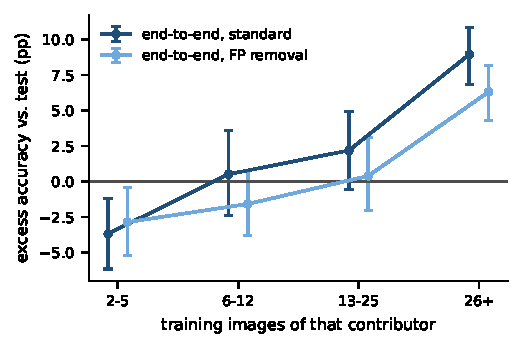
\includegraphics[width=\columnwidth]{fig_exposure}
\caption{Exposure dose--response of the end-to-end models: excess accuracy on new trips of seen
contributors, relative to the same countries' accuracy on unseen contributors, by the contributor's number
of training images; 95\% contributor-bootstrap CIs.}
\label{fig:exposure}
\end{figure}

\paragraph{Retrieval.} With 1-NN on the final partially fine-tuned features, 6.9\% of \tsh\ images find a
photo by the same contributor as their nearest neighbour in \vsh. These are 90.6\% correct, against
22.0\% for the rest, which explains about 4.7\pp\ of the 1-NN classifier's 6.7\pp\ gap. Frozen features
show the same pattern (5.0\% of queries; 89.6\% against 7.0\% correct). The end-to-end model behaves
alike: 6.3\% of queries retrieve the same contributor, those are 91.2\% correct against 21.2\%, worth
$0.063\times(0.912-0.212)\approx4.4$\pp\ of a 5.0\pp\ 1-NN gap. Fingerprint removal lowers the share of
same-contributor neighbours to 3.9\% (still 92.5\% correct), worth about 3.0\pp, and the 1-NN gap to
2.1\pp. The mechanism is unchanged; it simply fires less often.

\paragraph{Photographer verification.} The proposed classifier that predicts the contributor from the
features fails, since held-out contributors have at most four training images, so we test instead
whether images by the same photographer from different trips are more similar (cosine) than images by
different photographers from the same country. The area under the ROC curve (0.5 is chance) is 0.59
(test) and 0.62 (\tsh) for frozen features, and 0.57 for both the partially and the end-to-end
fine-tuned models. With fingerprint removal it falls to 0.55 on test and 0.56 on \tsh, and the share of
images whose nearest neighbour in the same split is by the same photographer falls from 14.0\% to 9.5\% on
test (random pairs: 0.1\%). Photographer style is visible in every representation, most in the frozen one,
yet only a classifier fitted to the training contributors converts it into a gap; fingerprint removal
makes the features measurably less photographer-specific, including for photographers never seen.

\paragraph{Where in the image.} Grad-CAM (Selvaraju et al.) on the last stage shows where the evidence for
the predicted class lies (Figure~\ref{fig:gradcam}). On 1{,}600 images (25 per country from test and from
\tsh), the final partially fine-tuned model puts 19.5\% (s.e.\ 0.2) of its evidence in the bottom 20\% of the
frame (20.3\% of the area), 12.9\% in the top quarter (sky) and 33.9\% in the central quarter; the end-to-end
model 19.7\%, 13.8\% and 37.1\%. The bottom band receives almost exactly its share of the area, slightly more
on \tsh\ than on test (20.0\% against 19.0\%), and the maps point to vegetation, buildings, poles and road
edges rather than to the bonnet. With fingerprint removal, which sees the band blanked, its share falls
to 17.0\% (the coarse $4\times6$ map spills into the band), and the top quarter rises from 13.8\% to 16.9\%.
Grad-CAM shows where the evidence for the \emph{predicted country} lies, not where the photographer
signal lies; that the bonnet is not a hot spot is consistent with the band mattering mainly for seen
photographers, as the blanking experiments below show.

\begin{figure*}[!t]
\centering
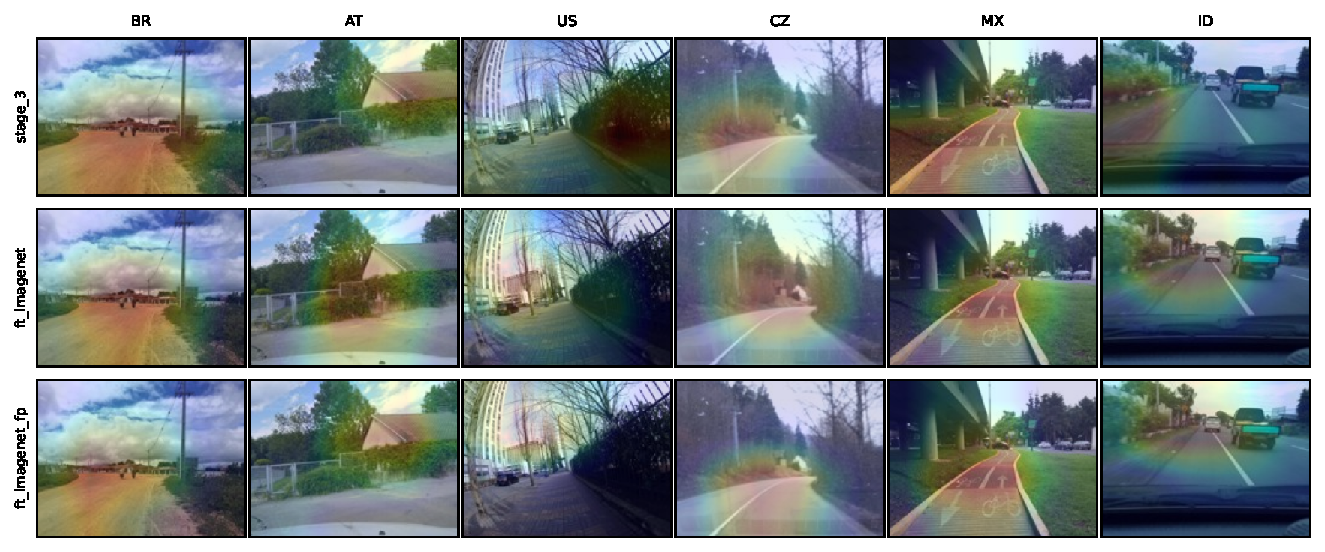
\includegraphics[width=\textwidth]{gradcam_panel}
\caption{Grad-CAM maps of the predicted class for test-set images (country codes above). Photos:
OSV-5M / Mapillary contributors, CC BY-SA 4.0.}
\label{fig:gradcam}
\end{figure*}

\section{Removing the Camera Fingerprint}
\paragraph{At test time.} Blanking the bottom 20\% of every evaluation image, without retraining, lowers
the final partially fine-tuned model's BA from 30.7\% to 20.9\% on unseen contributors and from 38.0\% to
23.9\% on seen ones. On the same bootstrap draws, test BA changes by $-9.8$\pp\ [$-10.8$, $-8.8$] and the gap
by $-4.3$\pp\ [$-5.8$, $-2.9$], to $+3.0$\pp\ [1.6, 4.5]. For the end-to-end model, test BA changes by
$-9.2$\pp\ [$-10.2$, $-8.3$] and the gap by $-2.4$\pp\ [$-3.8$, $-1.1$], to $+2.7$\pp. The band holds about
58\% and 46\% of the two gaps but only about a third of the accuracy, so both models read the bonnet and
dashboard disproportionately for photographers they know. The accuracy loss mixes two effects that this
experiment cannot separate: information removed and a distribution shift, since neither model saw a
blanked image in training.

\paragraph{During training.} Trained with fingerprint removal, the end-to-end model reaches 28.2\% on
unseen and 31.3\% on seen contributors, against 31.9\% and 37.0\% for the identical model trained without
it (Table~\ref{tab:main}, Figure~\ref{fig:e2e}a--b). On the same bootstrap draws, fingerprint removal changes
test BA by $-3.6$\pp\ [$-4.5$, $-2.8$], \tsh\ BA by $-5.7$\pp\ [$-6.6$, $-4.9$] and the gap by $-2.1$\pp\
[$-3.3$, $-0.9$], from $+5.2$ to $+3.1$\pp\ [1.3, 4.8]. Seen photographers lose more than unseen ones, which is
the signature of a shortcut being removed. The validation gap per epoch tells the same story: it opens
from $-0.3$ to $+3.9$\pp\ for the standard model as it fits the training set, but only from $-1.4$ to
$+1.8$\pp\ with fingerprint removal, whose training accuracy also stays lower (Figure~\ref{fig:e2e}c--d).

Per country (Figure~\ref{fig:countries}b), the gap shrinks in 21 of 32 countries, and the per-country gaps
of the two models remain highly correlated ($r=0.91$): fingerprint removal scales the shortcut down rather
than moving it. It shrinks most where it was largest ($r=0.61$ between a country's gap and its reduction):
Thailand ($-12.2$\pp), Denmark ($-10.0$), Switzerland ($-6.2$), Mexico and Canada ($-5.5$ each) and Malaysia
($-5.0$). Croatia, Belgium, Hungary and Austria keep gaps of 10 to 15\pp, so their photographer cues lie
outside what the intervention touches. The accuracy cost is concentrated in Switzerland ($-8.3$\pp),
Thailand ($-7.5$), Mexico ($-7.3$), Sweden and Poland ($-7.0$ each) and the United States ($-6.8$). The bottom
fifth of a forward-facing frame is mostly road surface, and road markings, kerbs and surface colour are
genuine country cues, so the band carries country information as well as camera information. Errors also
become less geographic: 59.1\% stay in the right region against 62.1\%, and new cross-region confusions
appear (Mexico as Brazil, Russia as Sweden). Two countries stand out with strongly negative gaps under
both models, Taiwan ($-18$\pp) and India ($-14$\pp): their seen photographers' new trips are \emph{harder}
than unseen photographers' images. We read this as a composition effect, plausibly a few heavy
contributors whose training trips taught the model a narrow view of the country, but with 400 images per
country it is a hypothesis, not a finding.

\begin{figure*}[!t]
\centering
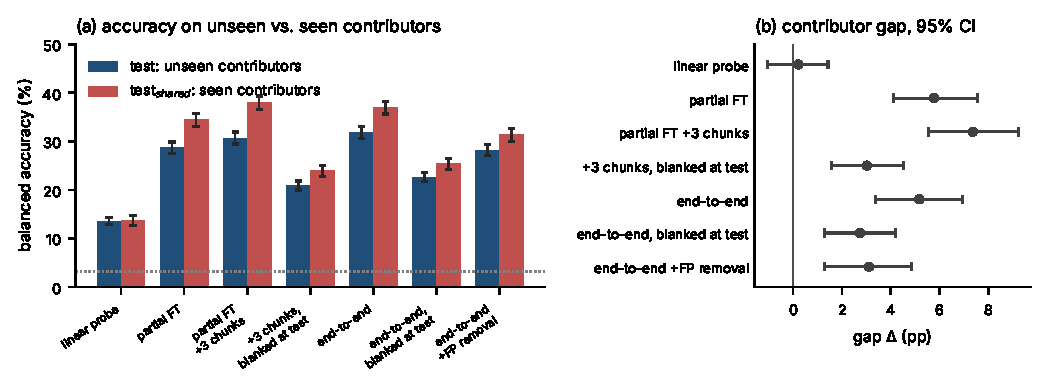
\includegraphics[width=\textwidth]{fig_e2e}\\[4pt]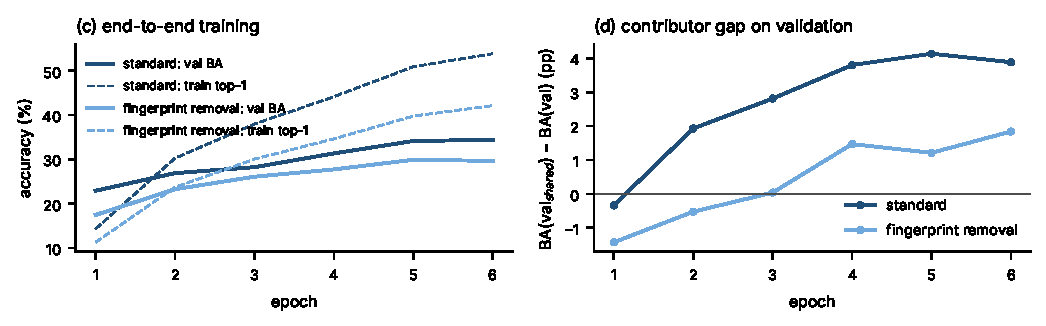
\includegraphics[width=\textwidth]{fig_curves}
\caption{(a) Balanced accuracy on unseen and seen contributors and (b) the contributor gap with 95\% CIs,
for all models and interventions. (c) End-to-end training curves and (d) the contributor gap on validation,
without and with fingerprint removal.}
\label{fig:e2e}
\end{figure*}

\paragraph{Combining the frames of a trip.} Averaging log-probabilities over the frames of a trip lifts the
final partially fine-tuned model from 30.7\% per image to 31.1\% [29.8, 32.3] per trip on test, because the
budgets leave most trips with one frame (10{,}658 trips for 12{,}800 images). On the 1{,}126 test trips with
two or more frames, accuracy rises from 32.2\% for single frames to 40.0\% for the trip, and from 33.9\% to
40.7\% for the end-to-end model: a few frames of one trip add about 7\pp, more than tripling the training
data did. Aggregation also amplifies the contributor gap. On \tsh\ the same models go from 37.3\% to 50.1\%
and from 36.9\% to 47.7\%, so on multi-frame trips the end-to-end model's gap grows from 3.0 to 7.0\pp;
with fingerprint removal it grows only from 1.2 to 3.8\pp\ (30.1\% to 36.4\% on test, 31.3\% to 40.2\% on
\tsh). Frames of one trip share the camera, so votes compound photographer evidence as well as country
evidence. The test and \tsh\ trip sets differ in country mix, so these gaps are indicative.

\section{Discussion}
\paragraph{Countries are learned.} On photographers it has never seen, the end-to-end ResNet-18 is right on
31.9\% of images over 32 countries, ten times chance; two-thirds of its errors stay in the right world
region, 70\% of left-hand-traffic images go to a left-hand-traffic country, and half its errors land within
about 2{,}500\,km. These are country cues, not camera cues, because they hold for unseen photographers.
The comparison of models shows where they come from: colour and gradient statistics carry little
(5.6\%), generic ImageNet features more (13.5\%), and most of the gain comes from adapting the network to
street scenes, which is also where the geographic structure of the errors appears.

\paragraph{Photographers are learned too.} The same network is 5.2\pp\ more accurate on new trips of
photographers it was trained on (7.4\pp\ for the partially fine-tuned model that saw more images of
them). Four observations place this gap in the contributors rather than in geography. It is absent from
frozen features and appears only when the classifier is fitted to the training contributors. It rises
with a contributor's number of training images, reaching about 9\pp\ for the most-seen contributors in
both training regimes. Most of it is carried by queries whose nearest neighbour is the same photographer.
And it shrinks when camera cues are removed, with seen photographers losing more accuracy than unseen
ones. Photographer style is decodable even from frozen ImageNet features (AUC 0.59 to 0.62), so the
representation always contains it; what creates the shortcut is optimisation on a training set in which
a contributor's images all carry the same label, the classic setting for shortcut learning (Geirhos et
al.): a camera that only ever drives in Thailand is a perfect, cheap feature for ``Thailand''.

\paragraph{More of the same data is not the cure.} Under a cap of 100 images per contributor the extra
261k images mostly repeat photographers already in training; they bought 2.0\pp\ on unseen contributors but
3.5\pp\ on seen ones. End-to-end training on the original 101k images beat the 363k-image model on unseen
contributors ($+1.2$\pp\ [0.4, 1.9]) with a smaller gap ($-2.2$\pp\ [$-3.3$, $-1.1$]). For crowd-sourced
geolocation data, the number of distinct contributors per country, not the number of images, is the
quantity to grow; our water-filling budgets, which spread each country's images over as many contributors
as possible, are a cheap way to do so.

\paragraph{Removing the camera has a price.} Fingerprint removal during training cuts the gap by about
40\%, and blanking at test time alone by about half, but neither closes it, and both cost accuracy on
unseen photographers (3.6 and 9.2\pp). The intervention removes country information along with camera
information, because the bottom of the frame shows the road as well as the bonnet, and the remaining gap
and the surviving dose--response show that photographer cues also live elsewhere: windscreen reflections
and mounts, the field of view and lens distortion (visible in several Grad-CAM examples), the height of the
horizon, and a contributor's habitual roads, seasons and times of day. Only some of these can be removed
by augmentation, and some (routes, seasons) are entangled with geography itself. Whether to apply it
depends on the goal: for the best accuracy on new photographers the standard end-to-end model is better;
for a model whose accuracy should not depend on who took the photo, fingerprint removal is the better
trade. If the camera is to be removed, it must be removed during training: blanking at test time reaches
a similar gap at two and a half times the accuracy cost.

\paragraph{Implications for benchmarks.} On the official OSV-5M split, 98.2\% of test images come from
training contributors, so published accuracies, including the 68.0\% of a fine-tuned ViT-L/14 (Astruc et
al.), mix country recognition with photographer recognition. Our gaps suggest that, for a ResNet-18 at low
resolution, the photographer part is worth several points of accuracy; since the gap grew with the number
of images per contributor, larger models trained on all 4.9M images, with far more images per
contributor, plausibly benefit more. We cannot measure this here, but it argues for reporting accuracy on
a contributor-disjoint test set next to the official one. Trip aggregation points the same way: votes over
a trip's frames add 7\pp, but they also double the seen-photographer advantage, so multi-frame evaluations
are even more exposed to the shortcut.

\paragraph{Issues and decisions.} Downloading the full OSV-5M archives would take about 245\,GB, so we
fetched single images by HTTP range requests. Without Kaggle GPU access, the CPU models froze the first
layers (10 to 17 images/s); the end-to-end models were trained at the end on a laptop GPU, where running
both at once made the machine swap and we switched to running them one after the other. The proposed
static-pixel masks found no camera pixels and were replaced by bottom-band blanking. The proposed
contributor classifier was replaced by pairwise verification because held-out contributors have too few
images to train one.

\paragraph{Limitations.} All runs use one seed and one split, and the CIs ignore model selection and
training randomness; the 2.1\pp\ effect of fingerprint removal is therefore a single paired comparison of
two training runs. The end-to-end models were trained for only 6 epochs, with the schedule shortened after
epoch 4, and the from-scratch pair of the planned
$\{$ImageNet, scratch$\}\times\{$standard, fingerprint removal$\}$ design was not run within our compute,
so we cannot say whether a network without ImageNet pre-training leans more or less on the camera. At
$128\times170$ pixels absolute accuracies are lower bounds, while $\Delta$, which compares two test sets
through one model, is less affected. The first data chunk added class weights together with new data.
Bottom-band blanking removes bonnets and dashboards but not windscreen reflections, mounts or colour
profiles, and its accuracy cost cannot be split between lost information and distribution shift. Country
labels come from GPS positions, and border label noise was not checked; the OSV-5M driving-side field marks
the United Kingdom as right-hand traffic, so we used real-world driving sides. The subset script is not
bit-reproducible across platforms (an unstable sort breaks ties between equally large trip groups
differently on x86 and ARM); the evaluation sets are therefore fixed by the committed prediction files,
and the end-to-end training set is a statistically equivalent re-draw that excludes every held-out trip.
Re-evaluating the released checkpoint on the new machine reproduces all 38{,}118 committed predictions
exactly.

\section{Conclusions and Future Work}
A ResNet-18 trained on crowd-sourced street views learns country cues that transfer to photographers it
has never seen: 31.9\% balanced accuracy over 32 countries after end-to-end fine-tuning, against 3.1\%
chance and 13.5\% for frozen ImageNet features, with errors that respect driving side and world region.
But part of what it learns is the photographers themselves: a contributor gap of $+5.2$\pp\ ($+7.4$\pp\
after more images of the same contributors) that frozen features do not show, that rises with a
contributor's exposure, and that retrieval of the same photographer explains. Training with fingerprint
removal reduces the gap by about 40\%, to $+3.1$\pp, and makes the features less photographer-specific, at
a cost of 3.6\pp\ on new photographers; the remaining gap shows that the camera is not only in the bonnet.
Contributor-disjoint evaluation, and more contributors rather than more images per contributor, should be
the default for geolocation models built from crowd-sourced data. The class game, \emph{Dashcam Duel}, lets
players compete against the final model, which gets 31\% of its 640 test photos right. Code and run
artefacts: \url{https://github.com/LaGuadana/country-not-camera}.

\paragraph{Future work.} Four extensions follow directly from our limitations. First, the from-scratch
pair of the planned design would show whether a network without ImageNet pre-training leans more or less
on the camera. Second, repeating every run over several seeds and contributor splits would turn the
single paired comparison of fingerprint removal into an estimate with training variance included. Third,
training at higher resolution would test our reading that the network misses fine cues such as signs,
plates and bollards, which separate neighbouring countries. Fourth, fingerprint removal could target the
remaining camera cues, such as field of view, lens distortion and horizon height, for example by random
crops and rescaling during training or by an adversarial loss that penalises features predictive of the
contributor.

\BAMunnumberedsection{Works Cited}
\begin{description}[leftmargin=2em,labelindent=0pt,font=\normalfont,itemsep=2pt]\small
\item Astruc, Guillaume, et al. ``OpenStreetView-5M: The Many Roads to Global Visual Geolocation.'' \emph{Proceedings of the IEEE/CVF Conference on Computer Vision and Pattern Recognition}, 2024, pp. 21967--77, https://doi.org/10.1109/CVPR52733.2024.02074.
\item Dalal, Navneet, and Bill Triggs. ``Histograms of Oriented Gradients for Human Detection.'' \emph{Proceedings of the IEEE Conference on Computer Vision and Pattern Recognition}, vol. 1, 2005, pp. 886--93.
\item Deng, Jia, et al. ``ImageNet: A Large-Scale Hierarchical Image Database.'' \emph{Proceedings of the IEEE Conference on Computer Vision and Pattern Recognition}, 2009, pp. 248--55.
\item Field, Christopher A., and Alan H. Welsh. ``Bootstrapping Clustered Data.'' \emph{Journal of the Royal Statistical Society: Series B (Statistical Methodology)}, vol. 69, no. 3, 2007, pp. 369--90.
\item Geirhos, Robert, et al. ``Shortcut Learning in Deep Neural Networks.'' \emph{Nature Machine Intelligence}, vol. 2, no. 11, 2020, pp. 665--73.
\item \emph{GeoGuessr}. GeoGuessr AB, www.geoguessr.com. Accessed 11 Oct. 2026.
\item Haas, Lukas, et al. ``PIGEON: Predicting Image Geolocations.'' \emph{Proceedings of the IEEE/CVF Conference on Computer Vision and Pattern Recognition}, 2024.
\item Hays, James, and Alexei A. Efros. ``IM2GPS: Estimating Geographic Information from a Single Image.'' \emph{Proceedings of the IEEE Conference on Computer Vision and Pattern Recognition}, 2008, pp. 1--8.
\item He, Kaiming, et al. ``Deep Residual Learning for Image Recognition.'' \emph{Proceedings of the IEEE Conference on Computer Vision and Pattern Recognition}, 2016, pp. 770--78.
\item Luk\'a\v{s}, Jan, et al. ``Digital Camera Identification from Sensor Pattern Noise.'' \emph{IEEE Transactions on Information Forensics and Security}, vol. 1, no. 2, 2006, pp. 205--14.
\item Selvaraju, Ramprasaath R., et al. ``Grad-CAM: Visual Explanations from Deep Networks via Gradient-Based Localization.'' \emph{Proceedings of the IEEE International Conference on Computer Vision}, 2017, pp. 618--26.
\item Torralba, Antonio, and Alexei A. Efros. ``Unbiased Look at Dataset Bias.'' \emph{Proceedings of the IEEE Conference on Computer Vision and Pattern Recognition}, 2011, pp. 1521--28.
\item Vivanco Cepeda, Vicente, et al. ``GeoCLIP: Clip-Inspired Alignment between Locations and Images for Effective Worldwide Geo-Localization.'' \emph{Advances in Neural Information Processing Systems}, vol. 36, 2023.
\item Weyand, Tobias, et al. ``PlaNet: Photo Geolocation with Convolutional Neural Networks.'' \emph{Proceedings of the European Conference on Computer Vision}, 2016.
\item Zech, John R., et al. ``Variable Generalization Performance of a Deep Learning Model to Detect Pneumonia in Chest Radiographs: A Cross-Sectional Study.'' \emph{PLOS Medicine}, vol. 15, no. 11, 2018, e1002683.
\end{description}

\section*{AI Acknowledgement}
Generative AI (Claude, Anthropic) was used in this project, in line with the course policy on AI use.
\pending{Team to confirm and complete:} it was used as a coding assistant to write and debug the data
pipeline, training and evaluation scripts; to port the training code to the laptop GPU and run the
final end-to-end experiments and analyses (test-time blanking, Grad-CAM, trip aggregation); and to draft
and edit report text. The research question, dataset choice, evaluation design and interpretation are
the team's; all numbers come from the scripts in the repository and were checked against the run outputs.
\end{document}
